\section{System Model}
Figure~\ref{fig:system_architecture} illustrates the overall architecture of the event-driven messaging system considered in this work. The system consists of four major components: (1) event producers, (2) ingest and queue services, (3) subscriber services, and (4) distributed consumer clients connected via persistent subscription transport connections.
\begin{figure*}[t]
	\centering
	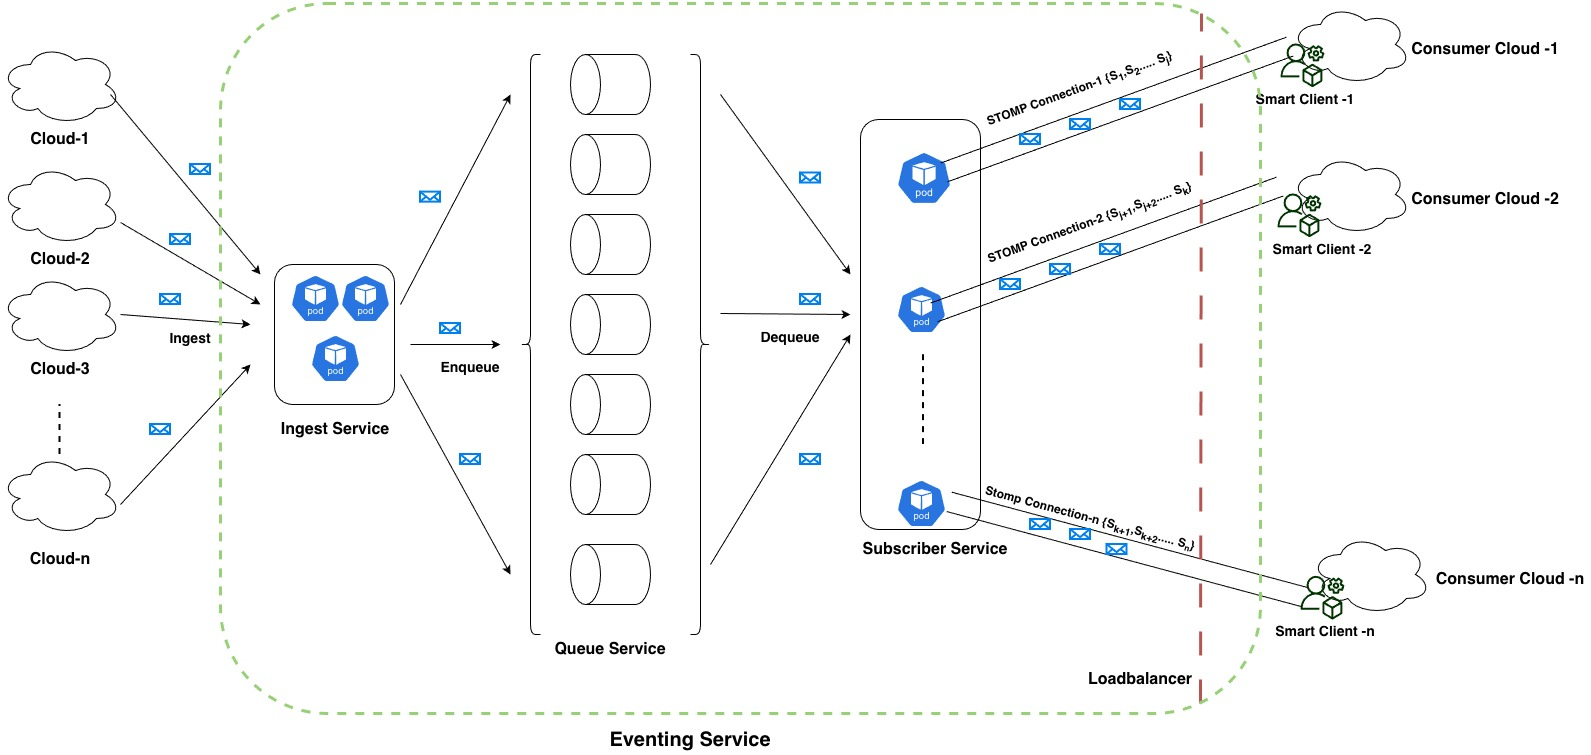
\includegraphics[width=\textwidth]{System-Architecture.jpg}
	\caption{System architecture with the DQL policy option shown. Producers send events through ingest services to durable subscription queues. Subscriber Pods deliver events over persistent connections. A client retains a load-balancer-assigned probe and promotes that same socket only after policy selection and execution checks. Greedy selection uses the same observation and actuation interfaces.}
	\Description{Left-to-right architecture diagram. Producer clouds send events through ingest pods into durable queues. Subscriber pods read those queues and accept persistent connections through a transport load balancer. On the right, a smart client maintains active connections, a subscription-free random probe, local queue metrics, a DQL controller, and a guarded action executor. Feedback arrows carry pod statistics to the client and connection operations back to the subscriber pods.}
	\label{fig:system_architecture}
\end{figure*}

\subsection{Event Producers and Ingest Service}

Event producers run in independent cloud environments, shown as Cloud-1 through Cloud-n in Figure~\ref{fig:system_architecture}. They generate events asynchronously and send them to the ingest service, which is the system's entry point.
The ingest service is implemented as a horizontally scalable set of service instances deployed as pods. Each ingest instance processes incoming events and enqueues them into the distributed queue service. The ingest service ensures reliable message intake and provides elasticity to handle fluctuating workloads.

\subsection{Queue Service}

The queue service acts as an intermediate buffering layer between event producers and subscribers. It provides durable storage and ensures reliable delivery of messages. Messages received from the ingest service are placed into queues, where they remain until consumed by subscriber services.The queue service supports parallel queues and can scale as event volume grows. Buffering lets producers and consumers work independently, without matching their processing rates.

\subsection{Subscriber Service}

The subscriber service is responsible for dequeuing messages from the queue service and delivering them to consumer clients. Similar to the ingest service, the subscriber service is deployed as multiple horizontally scalable instances.
Each subscriber service instance maintains persistent transport connections with multiple consumer clients. These connections may use STOMP-over-TCP, raw TCP, WebSocket, or another long-lived subscription-bearing transport. They allow real-time event delivery and enable clients to subscribe to specific event streams.
Subscriber service instances perform the following key functions:

\begin{itemize}
	\item Dequeue messages from the queue service
	\item Maintain subscription state for connected clients
	\item Deliver messages to subscribed clients
	\item Track subscription load, backlog, and delivery rate
\end{itemize}

The subscriber service instances are deployed behind a load balancer, which distributes incoming client connection requests across available subscriber instances.

\subsection{Load Balancer}

The load balancer serves as the initial connection routing layer between consumer clients and subscriber service instances. It distributes client connections across available subscriber instances using traditional transport-level algorithms such as round-robin or least-connections.

However, the load balancer operates without visibility into application-level metrics such as subscription count, message backlog, or processing load. As a result, connection assignments may not reflect the true load distribution across subscriber instances.
This limitation motivates the need for adaptive client-driven connection placement mechanisms.

\subsection{Consumer Clients and Persistent Transport Connections}

Consumer clients, referred to as Smart Clients in Figure~\ref{fig:system_architecture}, are deployed across multiple consumer cloud environments. These clients establish persistent subscription transport connections to subscriber service instances.

Each persistent transport connection can support multiple subscriptions. For
client $u$, let $\mathcal{K}_u(t)$ be its subscription set and
$\mathcal{C}_u(t)$ its active delivery-connection set. The subscriptions
assigned to connection $c\in\mathcal{C}_u(t)$ are

\begin{equation}
	\mathcal{K}_{u,c}(t)=\{k\in\mathcal{K}_u(t):z_{u,k,c}(t)=1\}.
\end{equation}

Here $z_{u,k,c}(t)$ is the binary assignment indicator defined in
Section~\mainref{sec:problem-formulation}. Each subscription corresponds to a
specific event stream or topic; $k$ indexes a subscription, not a Pod.

The subscriber service maintains subscription state and delivers messages to clients based on these subscriptions.
Because subscription counts and event rates may vary significantly across connections, the load imposed by each client connection is highly variable.

\subsection{Connection Placement and Rebalancing Model}

Let the set of subscriber service instances be denoted as:

\begin{equation}
	\mathcal{S}=\{1,2,\ldots,n\}.
\end{equation}

Each subscriber instance exposes the following dynamic statistics to active
connections and probe connections:

\begin{equation}
	y_i(t)=\bigl(p_i,X_i(t),B_i(t),H_i\bigr).
\end{equation}

where:

\begin{itemize}
	\item $p_i$ is the pod name
	\item $X_i(t)$ is the pod-level subscription count
	\item $B_i(t)$ is the cumulative backlog over all subscription queues served by the pod
	\item $H_i$ is the configured maximum processing threshold, used only as a capacity-normalization signal
\end{itemize}

These statistics are exposed to clients through protocol-specific statistics
frames, headers, or control messages. Actual drain behavior is measured from the client side using delivered,
processed, and acknowledged message counts, because the effective drain rate also depends on client processing capacity.

Decentralized monitoring research similarly treats telemetry quality and
monitoring overhead as coupled concerns. DEMon, for example, uses adaptive
gossip-based monitoring in volatile edge environments \cite{Ilager2026DEMon}.
Here the telemetry scope is deliberately smaller: active sockets and a retained
probe provide sampled Pod observations, not a complete cluster view.

Clients maintain persistent connections and periodically evaluate alternative subscriber instances using a learning-based placement and rebalancing strategy. Based on observed load characteristics, clients may rebalance subscriptions across their own connections, scale connection parallelism, or migrate subscriptions to alternative subscriber instances.This adaptive mechanism enables the system to dynamically rebalance load across client connections and subscriber service instances while operating only on client-visible statistics.

\subsection{System Characteristics}

The system exhibits the following important properties:

\begin{itemize}
	
	\item \textbf{Persistent connections.} Clients maintain long-lived STOMP-over-TCP,
	raw TCP, WebSocket, or equivalent subscription-bearing connections.
	
	\item \textbf{Subscription-Based Load:} Server load is determined primarily by subscription count and event rate, rather than connection count.
	
	\item \textbf{Dynamic Workload:} Event rates and subscription distributions change over time.
	
	\item \textbf{Distributed Architecture:} Subscriber services operate independently and scale horizontally.
	
	\item \textbf{Limited Load Balancer Visibility:} Load balancers lack application-level visibility into subscription load.
	
\end{itemize}

These characteristics make adaptive, client-driven connection placement particularly suitable for achieving optimal load balancing.




